\section{Introduction}
\label{sec:intro}

Pretrained Language Models (PLMs) have become popular in recent years and are used in many NLP tasks and applications.
An ongoing line of research is to understand how these models work, and analyzing what they can and cannot do.
For example, previous work showed that PLMs are very successful at capturing syntax, as was shown both in behavioral probes \cite{yoav-syntax} and structural probes \cite{structural-probe}.
On the other hand, other capabilities such as reasoning \cite{talmor2019olmpics}, commonsense \cite{Bosselut2019COMETCT,zhou2020evaluating} and world knowledge \cite{lama,jiang2020can} are moderate, and it has been questioned if these can be captured solely by PLMs at all \cite{Bender2020ClimbingTN}.


More recently, PLMs were suggested to be used as strong baselines for Knowledge Bases \cite{lama,jiang2020can}. Although the results of these models in the zero-shot setting outperform some supervised baselines, the results are still low, and the setup is limited (e.g. only reconstructing objects that consist of a single token, or the inability to return more than a single answer, or no answer whatsoever).
Yet, these studies lack an even more important property of KBs, that is \textit{consistency} and \textit{determinism}.
% \nk{I would add in this place a definition of the two terms}
% These properties require that the results returned from queries that are mapped into the same query in a KBs, will return the same results and in the same order.  
If two queries $q_1$ and $q_2$ are equivalent in the KB (e.g., if $q_1$ and $q_2$ are two equivalent ways to ask, in the formal language specified by the KB, for the retrieval of US presidents), they should return the same results, in the same order.
For example, consider the statement ```Homeland' was released on [MASK]'', where the `[MASK]' is the masked token that the model has to predict. We expect a model to predict the same answer with a pattern entailed by it: ``Homeland was aired on [MASK]'', e.g. \textit{Showtime}.
Note that in consistency, we do not expect the answers to be correct in the real world, which is a separate problem and has been addressed before, but for the predictions to be consistent, regardless of their true value.
These properties, although standard and well studied in classic KBs \cite{hansen2000probabilistic,Thimm:2009d,muino2011measuring}, are important for automatically constructed KBs.
% However, these properties were not studied in the context of LMs. 
However, it has not been studied to what extent PLMs used as KBs fulfill these requirements.
We note that consistency is largely \emph{independent} of accuracy, which is the property often studied: an inaccurate model can still err consistently, and it is possible that a specific PLM that is used as KBs is accurate \emph{only provided} it is queried in the ``correct" way, thus showing inconsistency when it is being used with semantically-equivalent natural-language queries.
Finally, these properties are important not only in the KBs usage, but in many other applications, such as Question Answering, Textual Entailment, etc, and was recently been addressed in the QA domain \cite{consistent-qa}. 


\begin{figure}[t!]
\centering

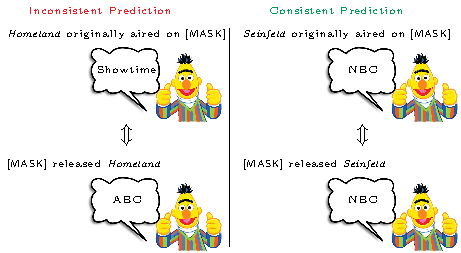
\includegraphics[width=1.\columnwidth]{figures/overview}

\caption{Overview of our approach. We begin with KB triplets (subject, pattern, object), of which we feed the (subject, pattern, [MASK]) into a PLM. 
We expect that a consistent model would predict the same answer for every two tuples of $(subject, pattern_1)$, $(subject, pattern_2)$ with an entailment connection between them. \nk{we should not use entailment but paraphrase connection right?}
\label{fig:overview}
% \vspace{-6mm}
\end{figure}




In this work, we propose a new benchmark to test consistency in LMs, using factual knowledge that was claimed to be partially encoded in PLMs.
This benchmark includes a manually curated resource, that provides sets of similar patterns -- short textual prompts that describe some relation \sr{similar in what sense?}.
Then, expecting from consistent models to predict the same answer for every two patterns with an entailment edge. \sr{the term ``entailment edge" is undefined at this point. Further, it is not clear what entailment even mean at this point in the intro.}
% We do so by conditioning on some factual knowledge statements that are stored by the model (the premise), and test whether the model correctly predict an inferred statement (the hypothesis).
An overview of our approach is displayed in Figure \ref{fig:overview}.




In order to test these capabilities, we manually build an Entailment Graph \cite{berant2011global,berant2012global,javad2018learning,hosseini2019duality} for each of the 41 relations in the T-REx dataset \cite{trex} provided by LAMA \cite{lama}, such as: \textit{born-in}, \textit{is-a-citizen}, \textit{works-for}, etc. 
These graphs were built by experts, and provide a high-quality resource, which we name \resource{}.
% \nk{jump from one graph to multiple graphs} 
Each of these graphs contains between @@-@@ different nodes, where each node is a pattern, e.g. ``[X] was aired on [Y]'', where \textit{[X]} and \textit{[Y]} are slot fillers for a subject and object.
These graphs are directional, which represent the entailment direction between two patterns (e.g. ``[X] was premiered on [Y]'' entails ``[X] was aired on [Y]'', but not the other way around).
Moreover, each edge is also annotated with the modification type (e.g. syntactic or lexical). %\nk{do we need to talk about syntactic and lexical here}.
% Moreover, the graphs also con the type of inference, such as lexical inference or syntactic inference \sr{I don't know re the term ``syntactic/lexical inference". Maybe focus on the alternations: ``we annotate the alternations between any pair of patterns as syntactic or lexical".}, which allows us to test different kinds of inference capabilities.
Examples of edges of the graphs are displayed in Table \ref{tab:rel-graph-examples}.



% Our framework \nk{the distinction between our data and the introduced framework is not clear here.} enables to test for consistency across different types of alternations in PLMs \nk{alternation is very vague}, and in this work, enabled by \resource{} we test for two prominent and basic capabilities: consistency over lexical and syntactic alternations. However, the framework is more general and allows to test other types of inferences, such as commonsense, pragmatics, etc. %\ar{Where is the boundary between lexical inference and commonsense inference}
% Moreover, by dissecting the consistency of PLMs, we provide a method to disentangle their inference capabilities, with those which are learned during training on some inference dataset, for instance, MNLI \cite{mnli}. 
% This will allow to better understand what kinds of capabilities a model learns during the pretraining step, and what it learns from a finetuning dataset. \sr{this sentence is redundant}
By evaluating the zero-shot consistency properties of models, we also allow inspecting these capabilities out-of-the-box, without adding finetuning biases. This allows to better understand what kinds of consistencies a model learns during pretraining, and will allow to track and improve this property in future work.


% By combining the \resource{} with the proposed framework, we are able to test different PLMs and how strong their consistency capabilities are.
Using \resource{}, we are able to probe for consistency in multiple PLMs.
We find that overall, current models perform poorly on the consistency benchmark, although there is a high variance between the different relations. 

Finally, we propose a method to boost the consistency capabilities of models, by continuing the pretraining with an additional consistency loss. Our results show promising results and achieve better consistency performance, but there's still a big gap before achieving consistent models.
